\chapter{微译器设计与实现}\label{chap:MUT}

上文\ref{sec:bt_overhead_all}我们通过分析发现二进制翻译器的主要开销来源于指令集语义差异和间接跳转开销。

指令集语义差异的一种常见的解决办法是在宿主指令集中添加指令集扩展,来接近客户指令集的语义,例如LoongArch指令中添加的二进制翻译扩展指令(Loongson Binary Translation, LBT)\cite{LoongArch2023}。
但这样会增加宿主指令集的复杂度,更加剧了指令集的历史包袱,同时添加指令集扩展也难以支持多种指令集的兼容。
我们从X86处理器定义的微码指令集中得到启发,微码是一种内部指令集,不对外暴露给用户和编译器,并且可以随着处理器的演进而不断迭代优化,不需要考虑历史兼容包袱。

我们希望能否定义一套\textbf{融合微码},作为一种内部指令集,包含各个指令集的并集,对外不暴露给用户,而是通过二进制翻译器将客户指令翻译为融合微码指令,从而实现多指令集的兼容。
在这个层面上,二进制翻译器类似于一个软件译码器,将客户指令翻译为融合微码指令,而CPU则类似于一个虚拟机,执行融合微码指令。
我们不太方便直接做一个硬件译码器,对外直接支持X86和RISCV等多个指令集,因为这样可能会面临X86授权问题。

而对于间接跳转开销,X86的微码缓存天然的就能解决这个问题,因为硬件上的微码缓存维护好了X86指令地址和微码指令地址的映射关系,可以通过简单的线性映射关系访问的微码指令地址,
而不需要软件上复杂的哈希表查询逻辑,这样可以大大减少间接跳转的开销。因此我们参考X86的微码缓存,提出了一种\textbf{翻译缓存}的概念,用于存储预翻译的融合微码指令集。
% 一条X86指令译码为多条微码指令,这个和一条宿主指令翻译为多条客户指令类似,都是一种一对多的关系。

为此我们借鉴X86微码和微码缓存的概念,提出了一种多架构软硬协同的二进制翻译技术——\textbf{微译器},
通过\textbf{融合微码}缩小了指令集语义差异,
通过\textbf{翻译缓存}来消除间接跳转开销,提高了二进制翻译器的性能。

\section{微译器整体架构}

\begin{figure}[!htbp]
  \centering
  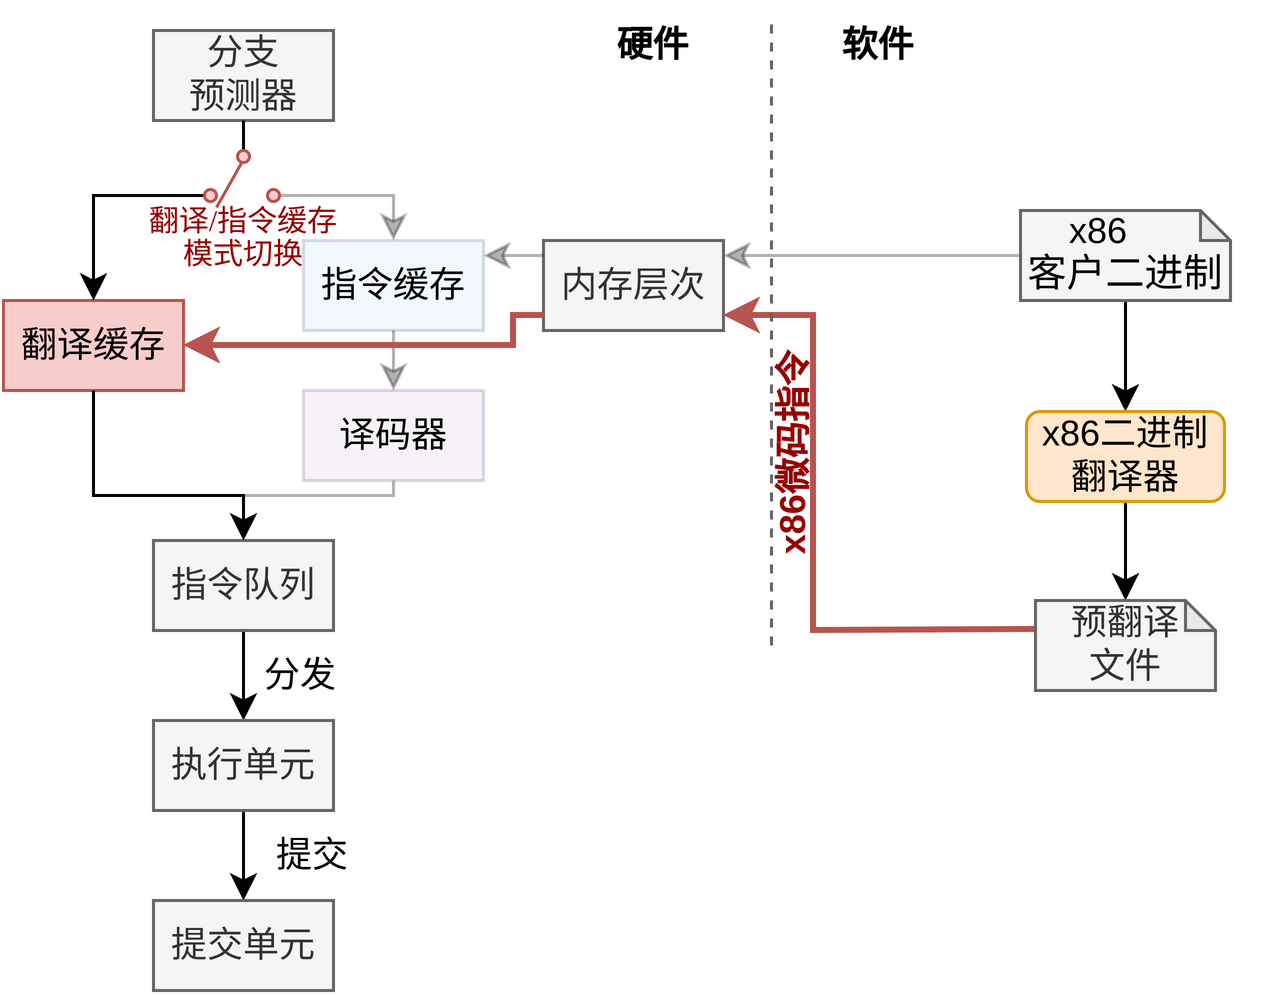
\includegraphics[width=1\linewidth]{./image/front_end_transutor.pdf}
  \caption{微译器整体架构图}
  \label{img:front_end_transutor}
\end{figure}

如图\ref{img:front_end_transutor}展示了微译器的整体架构,相对于传统的X86处理器前端图\ref{img:front_end_ucache},微译器在硬件侧和软件侧都做了一些改动。

% \subsection{硬件部分}

在硬件部分,引入了\textbf{翻译缓存}(Translation Cache),该缓存作为一级缓存负责存储预翻译的微码指令集,替代了原本的微码缓存。
翻译缓存的每行组织形式和微码缓存类似,都是前面部分存放微码指令(这里为融合微码指令,下一节详细介绍),
后面存放立即数,微码指令和立即数相向生长,中间可能有空洞,产生新的开销,后文会提出对应的优化方案。

此外与传统微码架构不同,微码缓存数据是直接来源于CPU和指令缓存,通过硬件译码器进行译码并存入微码缓存中;
而翻译缓存通过软件的二进制翻译“译码”,透过内存层次(从内存加载到L3 Cache, 再到L2Cache, 最后到微码缓存)进行填充,
取代了传统的指令缓存和译码器的角色。
在传统X86架构下,取指部件会同时查询指令缓存和微码缓存;
而在微译器架构下,取指部件仅查询翻译缓存,硬件的译码器被软件的二进制翻译器取代。
为了兼容传统的X86处理器模式,我们添加了一个模式切换逻辑,可以切换回使用硬件译码器进行译码,这样可以在不改变原有X86处理器的基础上实现微译器的功能。
后文我们默认使用软件二进制翻译器进行译码,也就是翻译缓存的方式。

% \subsection{软件部分}

在软件部分,引入了静态和动态二进制翻译器。
程序首先通过静态二进制翻译器被翻译成融合微码指令,并被写入预翻译文件,存储在硬盘中。
在客户程序执行阶段,预翻译文件被加载到内存中,程序计数器被设置为客户程序的入口。
取指部件从翻译缓存中取指,若翻译缓存或内存层次命中,则从翻译缓存取指,发送到处理器后端执行,不断取指执行。
若翻译缓存和内存层次均未命中(例如存在自修改代码等),说明客户指令还未翻译,此时会调用动态二进制翻译器进行实时翻译,
并将翻译结果写入翻译缓存,再取指执行。

接下来详细介绍微译器各个组成部分的设计与实现,包括融合微码、翻译缓存、预翻译文件、二进制翻译器。

\section{融合微码}\label{sec:tisa}
本节详细介绍重要的一个概念——融合微码。“融合”代表它能融合了多种指令集的特征,
包括X86和RISCV,未来还可以支持ARM,MIPS等其他指令集,
或许叫统一微码也更好理解。但融合并非简单的把所有指令集简单拼接就好,这会造成指令集冗余,挤占有限的编码空间。
而是需要对各个指令集的特征进行分析,找到共性,抽象出一种更加简洁的指令集,这就是融合微码的设计思想。

“微码”这个名字主要由于它在翻译缓存中的组织形式和传统的X86微码缓存组织形式类似,并且更像是不同指令集的更低级表现形式;
此外目前第一代的融合微码是在原有的Gem5 X86微码上扩充的,
所以便于理解仍然保留融合微码的名字。

但事实上,融合微码有很大特征很像一个“RISC指令集”。
由于我们的融合微码指令是需要存储在磁盘中的,并不像传统X86微码只是作为一个“暂时指令”存在于CPU运行期间,
所以融合微码指令需要像普通指令集一样进行\textbf{编码},
二进制翻译器把指令\textbf{编码}为定长的融合微码指令,并存储于磁盘中。
CPU再从磁盘中加载融合微码指令,\textbf{解码}为CPU识别的信息,这一阶段也叫“译码阶段”。
因此从这个角度来说,加上指令定长、只能操作寄存器、指令间关系被简化等特征,融合微码很像一个普通的“RISC指令集”。
因此融合微码类似传统指令集概念,也是有编码空间的概念。

\section{翻译缓存}\label{sec:tcache}

本节讲解翻译缓存的设计与实现,翻译缓存是微译器的核心组件,用于存储预翻译的融合微码指令集。

\begin{figure}[!htbp]
  \centering
  \includegraphics[width=1\linewidth]{./image/tcache_line.pdf}
  \caption{翻译缓存行组织形式}
  \label{img:tcache_line}
\end{figure}

翻译缓存的结构整体和微码缓存类似,但是有一些细节上的差异,这里我们详细介绍翻译缓存行的组织形式,
重点关注元信息和数据部分,其余的标签、有效位等部分和普通的一级缓存类似。
一篇关于微码缓存的专利\cite{uopPatent}中提到了微码缓存的一行设置为74byte。
而我们设计的翻译缓存行的大小为64字节,结构类似图\ref{img:ucache_line},但是元信息部分有所不同。

如图\ref{img:tcache_line},展示了翻译缓存行的组织形式,主要对元信息部分进行了详细介绍。
翻译缓存行的大小为64字节,
前16字节存放元信息,元信息细分为两部分,第一字节存放这一行的元信息,包括这一行是否有效,对应多少条宏码指令(这里的宏码就是客户指令,用宏码是为了和微码做对应)。
接下来15字节存放每条宏码的元信息,最多可以存15条宏码指令,宏码指令元信息包括宏码指令的长度(X86指令是变长指令,存储长度来索引到下一条X86指令地址),这条宏码生成的微码数量。
最后的48字节存放微码指令和立即数,微码指令和立即数都是定长的,单位为4字节。微码指令和立即数相向生长,中间可能有空洞。

存储行信息、微码指令、立即数是十分必要的,而存储宏指令元信息是为了支持二进制翻译器中精确异常处理。
精确异常处理是指在异常发生时,这条宏指令之前的所有指令都已经执行完毕,这条宏指令之后的所有指令都没有执行。
因此需要把一条宏指令对应的几条微码看做一个整体,可以乱序执行,但是在提交阶段需要保证这几条微码指令是原子提交的。
这样就能保证精确异常处理,这也是二进制翻译器必须要支持的功能。
因此在宏指令元信息中,需要存储一条宏指令对应的微码数量信息,而宏码长度信息则为了取到下一行微码缓存行。


\section{预翻译文件}\label{sec:aot}

本节讲解预翻译文件(Ahead-of-Time, AOT)的设计与实现,预翻译文件是存储预翻译的融合微码指令集的文件,是静态二进制翻译器的输出。

预翻译文件的设计思想在于,尽可能多的存储所有可能用到的融合微码指令,减少动态二进制翻译的开销。
由于融合微码和普通指令在一级缓存中寻址模式不同,普通指令能根据行内偏移直接访问到指令,而融合微码只能根据行内第一条指令的地址访问到整行指令(在\ref{sec:complex_isa}小节有提到)。
也就是说,融合微码只能以一个微码行(一个基本块)为单位进行访问,而不能以一个微码指令为单位进行访问。
如果出现了跳转到一个微码行的中间位置,那么就需要重新翻译这个微码行,这样会增加额外的开销。
对于传统的X86处理器模式,这个开销是很小的,因为是硬件来译码并填充到微码缓存中,只需要2拍左右;
而对于微译器架构,这个开销就会很大,因为需要调用软件的二进制翻译器进行实时翻译,可能需要上百拍的开销,这样的开销是无法接受的。
因此我们提出了\textbf{重复存储}的概念,即存储任意一个地址开始的融合微码指令,这样就能保证在跳转到任意一个地址时,都能从预翻译文件中加载对应的融合微码指令。


\section{二进制翻译器}

软件端的二进制翻译器分为静态二进制翻译器和动态二进制翻译器,静态二进制翻译器用于将客户程序翻译为融合微码指令,并存储在预翻译文件中;
动态二进制翻译器用于在翻译缓存未命中时实时翻译客户指令。

首先我们介绍静态二进制翻译器,它有如下3个设计目标:
\begin{enumerate}
  \item 可扩展性强:能够方便支持多种指令集的翻译。
  \item 代码发现性强:能够发现更多的二进制代码进行翻译,减少动态二进制翻译的介入。
  \item 可维护性强:能够方便的维护和更新翻译器。
\end{enumerate}

因此在实现上,如图\ref{img:mut_bt},我们尽可能的将翻译器的功能模块化,分为代码发现模块、反汇编模块、翻译模块、提交模块。
代码发现模块用于尽可能的发现更多的二进制代码,例如通过符号表、字符串表等信息发现更多的代码;
反汇编模块用于将ELF文件中的二进制代码转换为汇编代码;
翻译模块用于将汇编代码翻译为融合微码指令;
提交模块用于将翻译后的融合微码指令组织成翻译缓存行的形式,写入预翻译文件。

此外我们将架构相关的代码和架构无关的代码分开,架构相关的代码只有翻译模块,架构无关的代码主要是代码发现模块、反汇编模块和提交模块。
这样我们只需要添加新的翻译模块,就能够支持新的指令集的翻译,而不需要修改其他模块的代码。

最后我们希望尽可能复用现有的工具,例如LLVM objdump工具用于代码发现,这样能够减少二进制翻译器的实现难度,提高开发效率;
使用capstone工具用于反汇编,这样能够减少反汇编的实现难度,提高反汇编的准确性。
此外我们选用的LLVM objdump 和capstone工具都天然支持多种指令集,这样能够方便未来支持多种指令集的翻译。



\begin{figure}[!htbp]
  \centering
  \includegraphics[width=1\linewidth]{./image/mut_bt.pdf}
  \caption{静态二进制翻译器架构图}
  \label{img:mut_bt}
\end{figure}

而对于动态二进制翻译器,它的基本功能是在翻译缓存未命中时实时翻译客户指令,它和静态二进制翻译器的功能类似,
只是触发时机不同,因此我们可以复用静态二进制翻译器的代码,只需要添加一个触发机制即可。
它有两个触发机制,一个是代码发现没有发现的代码,需要实时翻译;一个是由于自修改代码等原因,翻译缓存行失效,需要实时翻译。
具体在硬件上,当翻译缓存行失效时,会触发例外(类似缺页异常),这时会调用动态二进制翻译器进行实时翻译,将翻译结果写入翻译缓存。